\documentclass[a4paper]{article}
\usepackage[T1]{fontenc}
\usepackage[utf8]{inputenc}
\usepackage[english]{babel}
\usepackage{amssymb}
\usepackage{hyperref}
\usepackage{mathtools}
\usepackage{amsthm}
\usepackage{varioref}
\usepackage{tikz}
\usetikzlibrary{positioning}

\tikzset{%
  every neuron/.style={
    circle,
    draw,
    minimum size=1cm
  },
  neuron missing/.style={
    draw=none, 
    scale=4,
    text height=0.333cm,
    execute at begin node=\color{black}$\vdots$
  },
}

\mathtoolsset{showonlyrefs}  
\hypersetup{
    colorlinks=true,
    linkcolor=black,
    filecolor=black,      
    urlcolor=black,
}

\setcounter{secnumdepth}{3}
\setcounter{tocdepth}{3}
\setlength{\parindent}{0pt}

\title{Urban sound classification}
\author{Francesco Tomaselli}
\makeindex
\begin{document}
\maketitle
\tableofcontents
\setlength{\parskip}{0.7em}
\newpage
\section{Introduction}

\emph{I declare that this material, which I now submit for assessment, 
is entirely my own work and has not been taken from the work of others, 
save and to the extent that such work has been cited and acknowledged within 
the text of my work. I understand that plagiarism, collusion, and copying 
are grave and serious offences in the university and accept the penalties that 
would be imposed should I engage in plagiarism, collusion or copying. 
This assignment, or any part of it, has not been previously submitted by 
me or any other person for assessment on this or any other course of study.}

The goal of this project is to build a neural network to classify audio 
files from the \emph{UrbanSound8k} dataset~\cite{dataset}.

This dataset contains audio divided in ten classes, each one representing 
a different type of city sound, for instance, we can find \emph{car horns}, 
\emph{dogs barking}, \emph{sirens}, etc. A deeper discussion about 
the dataset is present in the Subsection \vref*{dataset-structure}.

The presented methodology is composed of three main parts.
The first step is to extract relevant features from audio files using the
\emph{Librosa} library~\cite{librosa}.  This is discussed on Section 
\vref*{feature-extraction}.\\
The next step consists in composing and refining a neural network 
to classify the data obtained from the previous step. This part is 
made possible by the \emph{Keras} library and it is discussed in 
Section \vref*{model-definition}~\cite{keras}.\\
Lastly, results from the classification, namely accuracy 
and standard deviation among test sets, are presented in 
Section \vref*{results}.

The project is developed in \emph{Python} and the code is structured in 
a \emph{src} package~\cite{python}. Each one of the sub-packages contains code to deal 
with the different parts of the project. For instance, the \emph{data} folder 
contains the classes to extract features and to manage a dataset.

In addition to the package there is a \emph{notebook} folder containing
the different steps of the project and the various experiments made.

\newpage
\section{Feature extraction}
\label{feature-extraction}

This Sections presents the original dataset structure and the 
steps followed to create training and test sets from it.

Note that the models mentioned in this section, for the first and 
extended datasets are
three layers \emph{multilayer perceptrons}, 
a feed forward neural network where each layer 
is densely connected  to the following, 
with a reasonable number of neurons, trained 
for 100 epochs with default parameters for the \emph{stochastic gradient 
descent optimizer}.~\cite{mlp}\cite{sgd}\\
A \emph{convolutional neural network}, a network with 
a series of convolutional and pooling layers, followed by 
some densely connected ones, is applied to the image dataset, trained for 15 epochs
with default parameters for the Adam optimizer.~\cite{cnn} \\
For all datasets, the accuracy mentioned is computed with a \emph{cross-validation} 
approach.~\cite{cross}\\

A deeper discussion about the models structure as well as the validation
techniques used in the project can be found at Section \vref{model-definition}.

\subsection{Dataset structure}
\label{dataset-structure}

The UrbanSound8k dataset contains ten folds of audio samples, each one about 
four seconds long. The samples are divided in ten classes.\\
From the total of ten folds, the number one, two, three, four and six 
are taken as a training set, the others are each one a test set.
For this reason the following count about class numerosity considers
only the five training folds.

\begin{center}
    \begin{tabular}{ |l|c| } 
        \hline
        Class name & Number of samples \\
        \hline
        air conditioner & 500 \\
        car horn & 208 \\
        children playing & 500 \\
        dog bark & 500 \\
        drilling & 500 \\
        engine idling & 517 \\
        gun shot & 190 \\
        jackhammer & 548 \\
        siren & 536 \\
        street music & 500 \\
        \hline
    \end{tabular}
\end{center}

The table shows a clear class imbalance. In particular, the classes 
\emph{car horn} and \emph{gun shot} are not as numerous as the others. 
This can lead to poor performances on the these two categories, it is
therefore taken 
into consideration with training. 

The following table shows the number of samples in the training set and 
the various test sets.

\begin{center}
    \begin{tabular}{ |l|c| } 
        \hline
        Dataset & Number of samples \\
        \hline
        Training set & 4499 \\
        Test set 5 & 936 \\
        Test set 7 & 838 \\
        Test set 8 & 806 \\
        Test set 9 & 816 \\
        Test set 10 & 837 \\
        \hline
    \end{tabular}
\end{center}
All the operations on the datasets are performed with \emph{Pandas} library.~\cite{pandas}

\subsection{First dataset}
\label{first}
Extracting features from audio files is not straightforward, nonetheless there 
are a collection of audio characteristics that are commonly used in audio machine learning 
applications.~\cite{features}

To extract information from audio files \emph{Librosa} is used.~\cite{librosa}
The library provides many methods to choose from,
to keep it simple, for the first try with this dataset, the extracted features 
are these three ones: 
\begin{enumerate}
    \item \emph{Mel-frequency cepstral coefficients}: the first 20 coefficients 
    are extracted;
    \item \emph{Chromagram}: the first 12 chromas are considered;
    \item \emph{Root-mean-square}.
\end{enumerate}
Method parameters that are not specified in the above list, are left on their default values.
Each feature consists of an array of arrays containing measurements. 
A series of functions are applied to each sub-array and results 
are concatenated in a final feature vector. 
The functions applied are \emph{minimum}, \emph{maximum}, \emph{mean} 
and \emph{median} from the \emph{Numpy} library.~\cite{numpy}

This approach results in 132 components feature vectors.

\paragraph{Parallelizing feature extraction}
Extracting the three features listed above is really intensive 
but the task is easily parallelizable, in fact, each file is independent 
from one another.

For this purpose \emph{Dask} is used to speed up the computation and 
extract features from audio files in a multi-processing fashion.~\cite{dask}
The main idea is to build an execution plan, where each audio file 
is managed in parallel by a collection of workers. 
Improvement is great as the time to process a single fold 
is cutted into a third.

\paragraph{Feature scaling}
After testing some neural networks on the first dataset results 
are not promising. One of the reasons is the big difference in 
ranges among feature vector components, for instance, 
some audio characteristics are in the order of thousands while others 
range between zero and one.

To mitigate this effect a \emph{StandardScaler} with default parameters from \emph{scikit learn} is applied.~\cite{scaler}
The result is a dataset where each feature has more or less a distribution 
centered in zero with unit variance.
This leads to an improvement on the results using the same
model as before. 


\subsection{Extended dataset}
\label{extended-dataset}

Results using the three features named in the previous Subsection 
are promising but not enough, thus, to improve accuracy on the training set, 
new audio characteristics are extracted, namely:
\begin{enumerate}
    \item \emph{Zero-crossing rate};
    \item \emph{Roll-off frequency};
    \item \emph{Spectral flux onset strength}.
\end{enumerate}
As before methods parameters are left on default, but 
this time \emph{standard deviation} is added to
the previous functions \emph{minimum}, \emph{maximum}, \emph{mean} 
and \emph{median}. Each one is applied to the feature sub-vectors and 
results are concatenated, leading to a total of 180 features for each audio file.
Scaling yields to promising results on the first dataset, 
so the same approach is applied to the extended one.

After testing a network on the new training set 
we can see a better accuracy.

\paragraph{Feature selection}
Adding new features can lead to better results 
in the end but they all need to be useful to the model.
For this reason the extended dataset is subject of some experiments 
with feature selection, in particular \emph{PCA} algorithm from scikit
learn is applied.~\cite{pca}

The main idea is to select a reduced number of features from the total, 
loosing as little information as possible. This approach often leads to better results, 
as useless features are discarded.

The method used to select features offers the possibility to specify how much 
variance to preserve in the reduced dataset, this means that the number of 
components is not given explicitly, indeed we try to preserve 99 percent of the original variance.

This technique resulted in 102 features, unfortunately, a model applied to this new dataset 
failed to reach the performances obtained by the previous one, nonetheless, performances
improved with respect to the scaled dataset.

\subsection{Image dataset}
A completely different approach is followed this time to represent audio files 
as images, to later apply a convolutional neural network.

\paragraph{Audio as an image}
Representing an audio as an image is not straightforward but can be done after 
some preprocessing.
The main idea is to use audio features and consider them in a two dimensional 
space, where the value of a single cell can be viewed as a pixel.
Note that some features are well suited for this kind of representation, for instance, 
some of the previously extracted ones are given in output as a two dimensional vector.

Usually, an image has three channels, red, green and blue, but 
image classification on grayscale images, with one single channel 
is also relevant. This means that one can extract multiple features and view them 
as different channels, or choose only one to have the equivalent of a grayscale image.

\paragraph{Short time Furier Transform}
For this try with image classification the Short-time Furier transform 
is extracted from the audio files, and then used as a single channel image. 
In particular, we extract 128 intervals with the \emph{stft} function from Librosa, and, to accomodate 
the different lenghts of audio in the dataset, pad the result to 256 wide vectors.
The result is an $128 \times 256$ image for each sample. Figure \ref{img}
shows an example of an image obtained for each class.

\begin{figure}
    \includegraphics[width=\textwidth]{images/class_images.png}  
    \caption{Short time Furier transform on samples coming from each class.
    The scale on the Y axis is logarithmic, the X axis represent time and 
    the black portion on the edges is due to the applied padding.}  
    \label{img}
\end{figure}

We can see some difference between the classes, for instance, the \emph{dog barking}
shows short repeated sounds while \emph{air conditioner}
is constant. The hope is that those subtle differences are enough lo learn and classify.

\paragraph{Scaling pixel values}
Scaling techniques  are usually applied even to images to prevent high disparities 
among pixel value ranges, for this reason a Standard scaler with default parameters is 
once again applied to the training set to mitigate this effect.
We can not apply it directly to the images, as they are two dimensional, but we can 
flatten the pixel arrays, apply scaling and reshape them in the original $128 \times 256$ format.

Testing a convolutional network 
on the image dataset gives results that are comparable to the ones obtained on the initial scaled training 
set, discussed at Subsection \vref{first}.
\newpage
\section{Model definition}
\label{model-definition}

This Section starts by presenting how the networks used on the initial training sets are 
structured. We proceed to give a detailed overview of the performances 
on the different training sets, lastly, the hyperparameter tuning phase
is described.

\subsection{Neural network structure}
The starting point for the neural network structure is a 
reasonable network in terms of hidden neurons to prevent over-fitting, 
indeed a high number of units in the hidden layers would end up in learning 
too much from the dataset, leading to poor performances on the test sets.

For this reason, the rule of thumb followed to decide hidden neurons quantity is the 
following: 
$$\#\mathit{hidden\; neurons} = \frac{2}{3}\big(\#\mathit{input\;neurons}
+ \#\mathit{output\;neurons}\big)$$
The next step is to decide the hidden layers number. As using the rule 
presented above gives a quite small amount of units, only two layers are considered,  
indeed, an higher quantity would mean having a real small number of neurons per layer.

Applying this rule ended up in the following architectures on the four 
different training sets, where the output layer is fixed at 10:
\begin{center}
    \begin{tabular}{ |l|r|r|r| } 
        \hline
        Training set & Input & 1st Hidden & 2nd Hidden  \\
        \hline
        132 features unscaled &  132 & 60 & 30 \\
        132 features scaled &  132 & 60 & 30 \\
        180 features scaled &  180 & 80 & 46 \\
        102 features reduced with PCA &  102 & 45 & 30 \\
        \hline
    \end{tabular}
\end{center}

To build the actual model \emph{Tensorflow} and \emph{Keras} libraries 
are used.~\cite{tensorflow}\cite{keras}

\paragraph{Starting point model}
To give reference, this is the model used on the PCA training set, mentioned at 
the end of Subsection \vref{extended-dataset}, with 
102 input features.
\begin{center}
    
    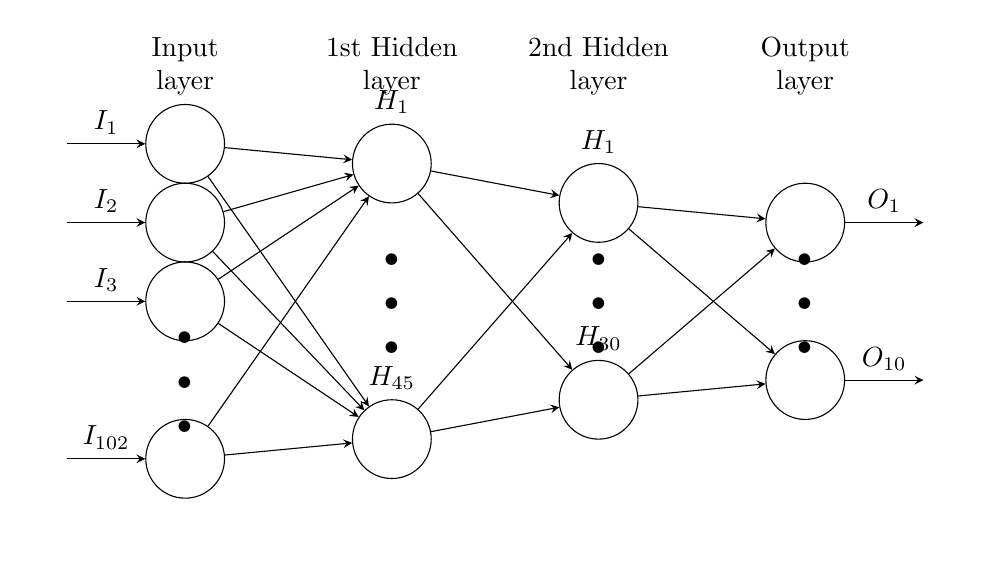
\begin{tikzpicture}[x=1.5cm, y=1cm, >=stealth]
        
        % layers
        \foreach \m/\l [count=\y] in {1,2,3,missing,4}
        \node [every neuron/.try, neuron \m/.try] (input-\m) at (0,2.5-\y) {};
        
        \foreach \m [count=\y] in {1,missing,2}
        \node [every neuron/.try, neuron \m/.try ] (hidden-\m) at (1.75,3-\y*1.75) {};
        
        \foreach \m [count=\y] in {1,missing,2}
        \node [every neuron/.try, neuron \m/.try ] (hidden2-\m) at (3.5,2-\y*1.25) {};
        
        \foreach \m [count=\y] in {1,missing,2}
        \node [every neuron/.try, neuron \m/.try ] (output-\m) at (5.25,1.5-\y) {};
        
        %   label
        \foreach \l [count=\i] in {1,2,3,{102}}
        \draw [<-] (input-\i) -- ++(-1,0)
        node [above, midway] {$I_{\l}$};
        
        \foreach \l [count=\i] in {1,45}
        \node [above] at (hidden-\i.north) {$H_{\l}$};
        
        \foreach \l [count=\i] in {1,30}
        \node [above] at (hidden2-\i.north) {$H_{\l}$};
        
        \foreach \l [count=\i] in {1,10}
        \draw [->] (output-\i) -- ++(1,0)
        node [above, midway] {$O_{\l}$};
        
        \foreach \i in {1,...,4}
        \foreach \j in {1,...,2}
        \draw [->] (input-\i) -- (hidden-\j);
        
        \foreach \i in {1,...,2}
        \foreach \j in {1,...,2}
        \draw [->] (hidden-\i) -- (hidden2-\j);
        
        \foreach \i in {1,...,2}
        \foreach \j in {1,...,2}
        \draw [->] (hidden2-\i) -- (output-\j);
        
        \foreach \l [count=\x from 0] in {Input, 1st Hidden, 2nd Hidden, Output}
        \node [align=center, above] at (\x*1.75,2) {\l \\ layer};
        
    \end{tikzpicture}
\end{center}
This last model, with the one built to predict the 180 features training set, are the ones selected for 
the hyperparameter tuning phase. 

\paragraph{Activation and loss functions}
The activation function for the input and hidden layers is a \emph{Relu}, 
typically used to prevent the \emph{vanishing gradient problem}, 
and the output one uses a \emph{Softmax} to have classification probabilities
among classes.~\cite{relu}\cite{soft}\cite{vanishing}\\
The loss used is the \emph{Sparse Categorical Crossentropy loss} as it 
is well suited for multiclass classification and, since 
the classes are integers and not one-hot encoded, the sparse version is preferred.~\cite{entropy}

\paragraph{Choosing an optimizer}
When choosing an optimizer for a neural network one must take into account the 
cost of reaching a minimum point on the error function.
Although more complex optimizers exist, build to reduce training 
cost or achieve better performances on deep networks, the one choosen 
for this model is a classic Stochastic Gradient Descent optimizer.

Testing some more advanced optimizers shows that convergence is reached faster on the 
networks used in the experiments, but the speed increase is negligible as the model
is quite small.

\subsection{Initial training set results}

Section \vref{feature-extraction} talks about the four different 
training sets obtained from the dataset and, without going into details, 
states that there is continuous improvement. 
We now give a more detailed look on training performances, after 
detailing how class imbalance is faced and the applied validation method.

Note that all the random seeds used by Tensorflow are fixed 
to make results reproducible. This step is necessary as many parameters initial 
value is random, for instance, the neural network weights.

\paragraph{Class imbalance}
To deal with the minority of some classes, balancing techniques should be 
applied when fitting the model. One of the possible approaches, and the one followed
here, is to assign class weights. 

The main idea is to penalize errors made on not well represented classes to account 
for their minority. Class weights computation relies on the \emph{compute class weights} function
from sklearn.~\cite{classweight}\\
The following are the computed quantities for the dataset classes:
\begin{center}
    \begin{tabular}{ |l|c|c| } 
        \hline
        Class name & Number of samples & Class weight \\
        \hline
        air conditioner & 500 & 0.8998 \\
        car horn & 208 & 2.1629 \\
        children playing & 500 & 0.8998 \\
        dog bark & 500 & 0.8998 \\
        drilling & 500 & 0.8998 \\
        engine idling & 517 & 0.8702 \\
        gun shot & 190 & 2.3678 \\
        jackhammer & 548 & 0.8209 \\
        siren & 536 & 0.8393 \\
        street music & 500 & 0.8998 \\
        \hline
    \end{tabular}
\end{center}
As expected, the less numerous classes have higher class weight than the rest,
in particular, the misclassification of a car horn sample
counts more than double than an air conditioner one.

\paragraph{Stratified cross-validation}
To estimate performance on the training set, stratified cross-validation with 
five folds is used. Basically the dataset is divided into five parts 
and a model is repeatedly trained on four and tested on one, all while considering class 
distribution, indeed, the original distribution of the classes is maintained 
in the splits.~\cite{stratified}

The stratified approach is required as there is class imbalance on the training set.
In fact, applying a classical cross-validation could show misleading results, 
for instance when the minority classes are more present 
in the test fold rather than the training ones; in such cases the loss would be 
higher.
The mean accuracy on the test folds gives a hint about the model performance.

For this step the \emph{Stratified KFold} class from scikit learn is used.~\cite{cross-scikit}

\paragraph{Results}
The following are the results on the training sets, using the architectures 
presented at the beginning of the Subsection.
\begin{center}
    \begin{tabular}{ |l|r|r| } 
        \hline
        Training set & Mean accuracy & St. deviation \\
        \hline
        132 features unscaled &  0.1138 & 0.0039 \\
        132 features scaled &  0.5743 & 0.0324 \\
        180 features scaled &  0.6363 & 0.0494 \\
        102 features reduced with PCA &  0.6188 & 0.0420 \\
        \hline
    \end{tabular}
\end{center}

There is a great improvement after scaling the training set, after 
that small refinements are made.
As accuracy is the best on the last two training sets, those are the two selected to 
perform the hyperparameter tuning.

\subsection{Hyperparameter tuning}

The last two tries with feature extraction lead to the best results 
with stratified cross-validation. Although the two models are reasonable, 
they can not be the final ones as many parameters are left on their default value, 
for instance, learning rate and momentum of the optimizer are untouched. 

The main goal now is to experiments with ranges of model parameters 
to find a better one. From now on, the model build on the 180 features training set is 
called \emph{Extended model}, 
while the one tested on the PCA training set is named \emph{PCA model}.

\paragraph{Grid and random search comparison}
Two of the most commonly used strategies in hyperparameter optimization
are \emph{grid} and \emph{random search}~\cite{random-grid}. 

In both cases we define ranges of parameters to test different combinations, 
for instance, fixed the number of neurons, one could try to find the best 
combination of learning rate and momentum that optimize accuracy on the training set.

While similar, the two methodologies differs in the amount of exploration they do.
The grid search try all the possible combinations of parameters, while the 
random approach fixes a number of iterations and picks an arbitrary unseen 
combination each time. 

Obviously the first one is more computationally expensive than the second, if 
we fix a small amount of possible iterations, but in theory it finds a better result
than going the random route. 
Nonetheless the grid search can led to over-fitting and in practice random 
search in preferred.

\paragraph{Random search}
We now run a random search with various parameters 
to optimize the initial models.
Note that class weights are still considered and the models are evaluated
again with a stratified cross-validation.
The optimizer used is the stochastic gradient descent.

The considered ranges for parameters for this run are: 
\begin{enumerate}
    \item \emph{Neurons}: input layer has dimension $H_i$ and last layer $H_o$, while 
    the two hidden layers are tested with a number of neurons respectively 
    equals to: 
    $$H_1 + 2i\;\;\text{and}\;\;H_2 + 2j,\;\;\text{with}\;\; i, j \in \{-2,-1,0,1,2\}$$
    \item \emph{Learning rate}: $0.001, 0.01, 0.1, 0.5$;
    \item \emph{Momentum}: $0.0, 0.01, 0.1, 1$;
    \item \emph{Epochs}: $60, 80, 100$;
    \item \emph{Batch size}: $32, 64$.
\end{enumerate}

Where $H_i$, $H_1$, $H_2$ and $H_o$ are input, first hidden, second hidden 
and output layer dimensions.
The random search is performed on two models, with those starting dimensions: 
\begin{itemize}
    \item \emph{Extended model}: 180, 80, 46, 10.
    \item \emph{PCA model}: 102, 45, 30 and 10;
\end{itemize}

An \emph{early stopper} with default parameters is used on the training to stop it when no progress is made with 
respect to the last epoch results.~\cite{early}
The search is performed with 100 iterations for both rounds.

\paragraph{Final models}
The first round of the random search, performed on the Extended model, resulted 
in the following parameters:
\begin{itemize}
    \item Neurons: 180 for input, 76 for the first hidden layer, 50 for the second and 10 for output;
    \item Momentum: 0.01
    \item Learning rate: 0.01
    \item Epochs: 80
    \item Batch size: 64
\end{itemize}
We can see an improvement in accuracy by comparing it with to starting point model:
\begin{center}
    \begin{tabular}{ |l|r|r| } 
        \hline
        Model & Mean accuracy & St. deviation \\
        \hline
        Initial extended model & 0.6363 & 0.0494\\
        Random search result & 0.6497 & 0.0431\\
        \hline
    \end{tabular}
\end{center}

The second random search on the smaller PCA model, resulted in this results:
\begin{itemize}
    \item Neurons: 102 for input, 45 for the first hidden layer, 30 for the second and 10 for output;
    \item Momentum: 0.01
    \item Learning rate: 0.1
    \item Epochs: 80
    \item Batch size: 32
\end{itemize}
As before, comparing it with the starting model, we can see some better results:
\begin{center}
    \begin{tabular}{ |l|r|r| } 
        \hline
        Model & Mean accuracy & St. deviation \\
        \hline
        Initial PCA model & 0.6188 & 0.0420\\
        Random search result & 0.6270 & 0.0315\\
        \hline
    \end{tabular}
\end{center}

\newpage
\section{Conclusions}
\label{results}

This last Section presents results obtained on the test sets. 
We test the best multilayer perceptron and the best convolutional network found.
As stated on the first Section, the five test sets are made out of the 
folds number five, seven, eight, nine and ten.

\subsection{Test set results}

\paragraph{Test set preprocessing}
The test sets are preprocessed with the same techniques used to extract the training sets.\\
In fact, regarding the MLP training set, the one with 180 features, all the features are extracted 
from the test audio files and scaled using the pre-fitted Standardscaler.
Similarly, each pixel in the test images is scaled using the Standardscaler 
fitted on the image training set.

\paragraph{Results}
The MLP model is the fine tuned one coming from the hyperparameter tuning phase, 
trained on the 180 features dataset, namely the \emph{Extended model}, 
while the CNN one is the best performer from the tried convolutional models, 
the so called $C_3$ network with 0.001 Adam learning rate and 32 batch size.
\begin{center}
    \begin{tabular}{ |l|r|r| } 
        \hline
        Test set & MLP Accuracy & CNN Accuracy\\
        \hline
        Fold 5 & 0.7425 & 0.5171\\
        Fold 7 & 0.6038 & 0.5668\\
        Fold 8 & 0.6873 & 0.5744\\
        Fold 9 & 0.6348 & 0.5515\\
        Fold 10 & 0.6858 & 0.5639\\ 
        \hline
    \end{tabular}
\end{center}

The mean accuracy and standard deviation are: 
\begin{center}
    \begin{tabular}{ |c|r|r| } 
        \hline
        Model & Mean accuracy & Standard deviation\\
        \hline
        MLP & 0.6708 & 0.0478 \\
        CNN & 0.5547 & 0.0202 \\
        \hline
    \end{tabular}
\end{center}

\subsection{Future works}

Results are better on MLP models, but CNNs
shows potential on the problem.
Results could be improved, indeed, 
a more refined training set creation can be made, by exploiting 
more features from the Librosa library, testing different type 
of scalers and experimenting with different feature selection 
techniques.

Regarding the image dataset, more channels could be considered 
by using more features as images, also, data augmentation techniques 
could be applied in order to increase the cardinality of the dataset.
Finally, with more computational power, a proper random search could be performed.
\input{chapters/conclusion.tex}

\newpage
\end{document}